\documentclass[crop, tikz]{standalone}
\usepackage{tikz}

\usetikzlibrary{positioning,decorations.pathmorphing}

\begin{document}
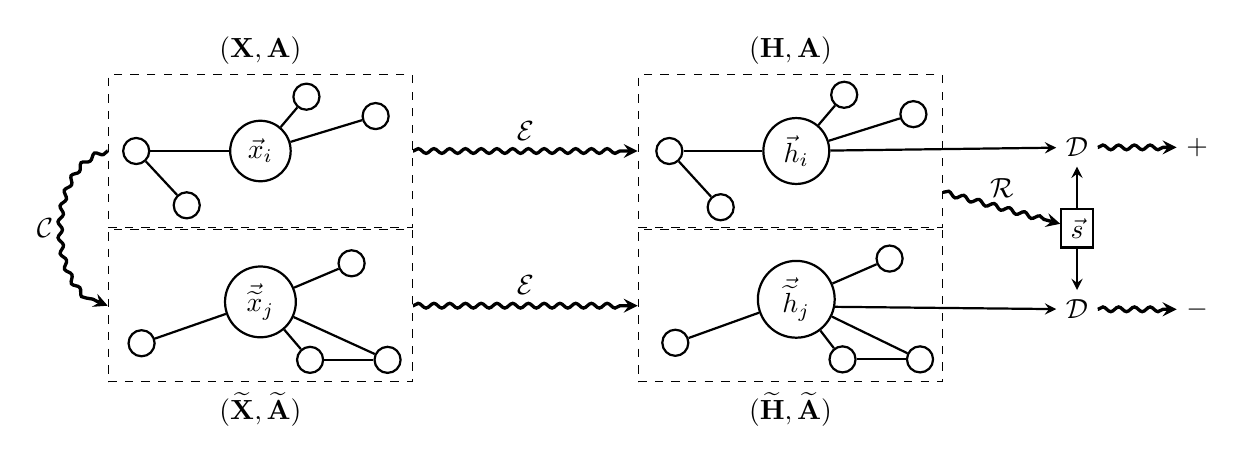
\begin{tikzpicture}
	\node[circle, thick, draw] (0) {$\vec{x}_i$};
	\node[circle, thick, draw, above right=0.1em and 3em of 0] (1) {};
	\node[circle, thick, draw, above right=0.8em and 0.5em of 0] (2) {};
	\node[circle, thick, draw, left=of 0] (3) {};
	\node[circle, thick, draw, below left=0.8em and 1.5em of 0] (4) {};
	
	\draw[-, thick] (0) -- (1);
	\draw[-, thick] (0) -- (2);
	\draw[-, thick] (0) -- (3);
	\draw[-, thick] (4) -- (3);
	
	\node[circle, thick, draw, below=3em of 0] (01) {$\vec{\widetilde{x}}_j$};
	\node[circle, thick, draw, above right=0.1em and 2em of 01] (02) {};
	\node[circle, thick, draw, below left=0.2em and 3em of 01] (03) {};
	\node[circle, thick, draw, below right=0.8em and 0.5em of 01] (04) {};
	\node[circle, thick, draw, below right=0.8em and 3.3em of 01] (05) {};
	
	\node[rectangle, draw, dashed, minimum width=11em, minimum height=5.5em] (RR) {};
	\node[rectangle, draw, dashed, minimum width=11em, minimum height=5.5em, below=0.05em of RR] (RR2) {};
	\node[above=0em of RR] (l1) {$({\bf X}, {\bf A})$};
	\node[below=0em of RR2] (l2) {$({\bf \widetilde{X}}, {\bf \widetilde{A}})$};
	
	\draw[-, thick] (01) -- (02);
	\draw[-, thick] (01) -- (03);
	\draw[-, thick] (01) -- (04);
	\draw[-, thick] (01) -- (05);
	\draw[-, thick] (04) -- (05);
	
	\node[rectangle, draw, dashed, minimum width=11em, minimum height=5.5em, right=12.5em of 0] (AA) {};
	
	\node[circle, thick, draw, right=17em of 0] (0) {$\vec{h}_i$};
	\node[circle, thick, draw, above right=0.1em and 3em of 0] (1) {};
	\node[circle, thick, draw, above right= 0.8em and 0.5em of 0] (2) {};
	\node[circle, thick, draw, left=of 0] (3) {};
	\node[circle, thick, draw, below left=0.8em and 1.5em of 0] (4) {};
	
	\draw[-, thick] (0) -- (1);
	\draw[-, thick] (0) -- (2);
	\draw[-, thick] (0) -- (3);
	\draw[-, thick] (4) -- (3);
	
	\node[circle, thick, draw, below=2.7em of 0] (01) {$\vec{\widetilde{h}}_j$};
	\node[circle, thick, draw, above right=0.1em and 2emof 01] (02) {};
	\node[circle, thick, draw, below left=0.2em and 3em of 01] (03) {};
	\node[circle, thick, draw, below right=0.8em and 0.3em of 01] (04) {};
	\node[circle, thick, draw, below right=0.8em and 3.1em of 01] (05) {};
	\node[rectangle, draw, minimum width=11em, minimum height=5.5em, dashed, below=0.05em of AA] (AA2) {};
	\node[above=0em of AA] (l1) {$({\bf H}, {\bf A})$};
	\node[below=0em of AA2] (l2) {$({\bf \widetilde{H}}, {\bf \widetilde{A}})$};
	
	\draw[-, thick] (01) -- (02);
	\draw[-, thick] (01) -- (03);
	\draw[-, thick] (01) -- (04);
	\draw[-, thick] (01) -- (05);
	\draw[-, thick] (04) -- (05);
	
	\draw[-stealth, very thick, decoration={snake, pre length=0.01mm, segment length=2mm, amplitude=0.3mm, post length=1.5mm}, decorate,] (RR) -- node[above] {$\mathcal{E}$} (AA);
	\draw[very thick] (RR.west) edge[bend right=75, decoration={snake, pre length=0.01mm, segment length=2mm, amplitude=0.3mm, post length=1.5mm}, decorate,-stealth] node[left] (CC) {$\mathcal{C}$} (RR2.west);
	\draw[-stealth, very thick, decoration={snake, pre length=0.01mm, segment length=2mm, amplitude=0.3mm, post length=1.5mm}, decorate,] (RR2) -- node[above] {$\mathcal{E}$} (AA2);
	
	\node[right=36em of CC, rectangle, draw, thick] (Re) {$\vec{s}$};
	
	\draw[-stealth, very thick, decoration={snake, pre length=0.01mm, segment length=2mm, amplitude=0.3mm, post length=1.5mm}, decorate,] (AA) -- node[above] {$\mathcal{R}$} (Re);
	
	\node[above=1.5em of Re] (D1) {$\mathcal{D}$};
	\node[below=1.5em of Re] (D2) {$\mathcal{D}$};
	
	\draw[-stealth, thick] (Re) -- (D1);
	\draw[-stealth, thick] (Re) -- (D2);
	\draw[-stealth, thick] (0) -- (D1);
	\draw[-stealth, thick] (01.-11) -- (D2);
	
	\node[right=of D1] (P) {$+$};
	\node[right=of D2] (M) {$-$};
	
	\draw[-stealth, very thick, decoration={snake, pre length=0.01mm, segment length=2mm, amplitude=0.3mm, post length=1.5mm}, decorate,] (D1) -- (P);
	\draw[-stealth, very thick, decoration={snake, pre length=0.01mm, segment length=2mm, amplitude=0.3mm, post length=1.5mm}, decorate,] (D2) -- (M);
	
\end{tikzpicture}
\end{document}